
\documentclass[a4, 10pt,dvipdfmx,twocolumn]{jsarticle}

%\usepackage[chukan]{sotsuron}
%\usepackage[dvips]{graphicx}

%\setlength{\topmargin}{-13truemm}
%\setlength{\headheight}{0mm}
%\setlength{\headsep}{0mm}
%\setlength{\textheight}{45\baselineskip}
%\setlength{\textheight}{26cm}
%\addtolength{\textheight}{\topskip}
%\addtolength{\textwidth}{5cm}
%\addtolength{\oddsidemargin}{-2.5cm}

\usepackage[dvipdfmx]{graphicx}
\def\pgfsysdriver{pgfsys-dvipdfmx.def}
\usepackage{threeparttable}
\usepackage{tikz}
\usepackage[chukan, nobroaderlayout]{sotsuron}
% \usepackage[chukan]{sotsuron}
\usepackage{ascmac}
\usepackage{bm}
\usepackage{amsmath}
\usepackage{fancybox}
\usepackage{url}

\title{モンテカルロ木探索を用いた交渉の評価関数の提案}
\author{東京大学工学部電子情報学科 近山,鶴岡研究室 4年 伊藤 義章}
\date{2013年9月30日}

\begin{document}
 % \makecover

\pagenumbering{roman}

 % \tableofcontents

\newpage
\maketitle

\pagenumbering{arabic}

\section{目的と背景}
実世界では多くの交渉が行われており、競争的状況において自分の利益を最大化することを目指している。このとき、お互いの利益を考慮した上で、先読みを行い自分の利益を最大化できる交渉を相手に提示し、自分にとって不利な交渉は受けないようにする必要がある。利益を最大化する交渉を探る手法の1つとして、実世界をモデル化した知能ゲームをコンピューターに解かせる方法がある。知能ゲームの研究は、情報システムによる支援など、実世界において実用的価値を持ちうるため、これを交渉にも適用する。
本研究では、これを現実社会に似たモデルである、カタンの開拓者(以下カタン)というマルチエージェント、非決定的、不完全情報なゲームを用いて評価測定を行う。このモデルで最適な交渉案を評価する関数(評価関数)を提示することで、現実世界での応用が期待できる。モンテカルロ木探索が先読みにおいて、有効な手段だという仮説のもと、互いの利益計算を行う。得られた利益に基づいて交渉の評価関数をいくつか列挙し、その中から自らの利益を最大化する評価関数を提案し、その有効性を測定する。
\section{関連研究}
\subsection{交渉}
一般的な競争型交渉は価格交渉のようにゼロサムゲームであり双方の損得は一致する。中には、双方の利益をふやすことができる場合があり、利益交換型交渉と呼ばれ、ゼロサムゲームよりも良い交渉形態である。この交渉を扱うことができることも、カタンで交渉研究する利点となる。
\subsection{UCTアルゴリズム (UCB applied to Trees)}
状態の評価が難しい問題において有効とされる手法としてモンテカルロ法がある。
ある局面から終局までランダムに行われる試行(プレイアウトと呼ばれる)に基づき、統計的に評価する。プレイアウトを繰り返す事で、ある局面の勝率を計算することができる。
しかし、有限な時間内に正確な勝率評価を行う場合、明らかに有望でない手に対して、有望な 手と同様の試行回数を行うべきではない。よって、これを解消するため有望な手にバイアスをかけて試行回数を配分する必要がある。これがUCBアルゴリズム (Upper Confidence Bound、以下 UCB) である\cite{kocsis2006bandit}。
子ノードを選択する場合、まず未探索の子ノードを優先的に選択する。
子ノードが全て探索済みの場合は、探索回数が少なく、高い報酬を得る可能
性のある手を優先的に選択する。
選択したノードをプレイアウトした後は、その結果を報酬として探索経路上のノードに更新する。
以上の「子ノードの選択」「子ノードの展開」「プレイアウト」「結果の更新」を終了条件 (時間や探索回数など) となるまで繰り返し、平均報酬の最も高い子ノードを次のアクションとする。
これらのアルゴリズムは、カタンのAIであるJSettlersに適用させ、成功をおさめている\cite{szita2010monte}。JSettlersのプレイヤーに対して、JSettlersをベースとしたモンテカルロ木探索で、0回シミュレート、1000回シミュレートおよび10000回シミュレートを行った。他の3人プレイヤーに対し、25\%、27\%、49\% の勝率を残し、カタンにおけるモンテカルロ木探索がランダムプレイヤーよりは強いことを示している。
本研究でも、UCTアルゴリズムをJSettlersで適用するものとする。
% \begin{figure}[b]
%     \begin{center}
%       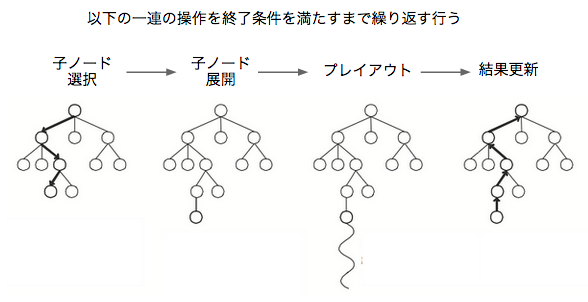
\includegraphics[width=80mm]{img/monte_carlo.png}
%     \end{center}
%     \caption{モンテカルロ木探索~\cite{kocsis2006bandit}}
%     \label{monte_carlo}
% \end{figure}
\section{提案手法}
\subsection{カタンの特徴と簡単化}
カタンには以下3つの特徴がある。
\begin{description}
\item[マルチエージェント]\mbox{}\\ 
全てのプレイヤーは自立的に行動し、複雑なアクションを行い、互いに影響を及ぼす。
本研究で交渉を行う時は、交渉を受けるプレイヤー間で影響を及ぼさないものとする。各プレイヤーに関して、1対1の最も良い交渉を選び、その中から最も良い交渉を提案する。
\item[非決定的]\mbox{}\\ 
サイコロとカードという確率的なモデルがあるため、探索する深さを増やしすぎると状態数が爆発してしまう可能性がある
\item[不完全情報]\mbox{}\\ 不完全情報だと考えられる状態数が急増する。本研究で完全情報としても測定に与える影響は少ないため、完全情報として近似して考えることにする。
\end{description}
\subsection{JSettlers}
JSettlersは、オープンソースなカタンのAIである。戦術はルールベースで、交渉時に相手が欲しい資源については考えない。そのため、お互いが満足する交渉が行われることは少ない。
本研究で、JSettlersを交渉の相手に使用する場合はまず、交渉を全く受けないプレイヤーと比較することで、JSettlersの交渉の有意性を示す必要が ある。その後、交渉を受ける相手としてJsettlersを設定し、妥当な交渉を検討していく。
\subsection{交渉の利益計算と評価関数の提案}
交渉を提案する上で自分と相手の利益を計算する必要がある。交渉を行った場合と交渉を行わなかった場合について、自分と相手の勝率を計算し、交渉を行った事による勝率の変化を利益(損失)として考える事にする。
さらに、相手プレイヤーが交渉に必ず応じるわけではないので、自分の利益を最大化しつつ相手に交渉に応じてもらう必要がある。
妥協点をみつけ出すために交渉内容の評価値を 以下のように設定する。
\\ \,\,\,\,\,\,\,(評価値) = (自分の利益)×(交渉成立確率)\\
交渉成立確率は相手の利益に比例する事が多く\\(交渉成立確率)=(相手の利益)として考える事にする。
本研究ではこの評価値が一番高い交渉内容を JSettlers を用いて検証する。特定のプレイヤーのみ、他のプレイヤーに対して毎ターン
交渉を行い、「交渉成立回数」「交渉に応じたときの評価値」「自分の勝率」の結果を比較する。
\section{おわりに}
\subsection{まとめ}
提案手法により、UCTを用いた先読みより得られた評価値に基づく交渉の評価関数の1つを得る事ができると期待される。また、今回シミュレーションを行うJSettlersの交渉時における挙動を確認できるため、今後の交渉相手として交渉を受け入れるプレイヤーであるかを確認できると期待される。
\subsection{進捗状況}
交渉を行うために、評価値を生成するUCTアルゴリズムの実装をJSettlersを動作させる環境を整備した。また、JSettlers上で動くUCTアルゴリズムの実装を現在行っている。実装を終えた後、評価値を用いて交渉を行う評価関数の生成に入る。
\subsection{今後の計画}
今後の課題は
% \begin{itemize}
%  \item 「様々な局面を用意し対戦実験を行い、UCTによる利益計算を行う」
%  \item 評価値に基づく交渉の評価関数を用意して、再度様々な局面に対する対戦実験を行い自分の利益を最大にする評価関数を調べる
% \end{itemize}
「様々な局面を用意し対戦実験を行い、UCTによる利益計算を行う」「評価値に基づく交渉の評価関数を用意して、再度様々な局面に対する対戦実験を行い自分の利益を最大にする評価関数を調べる」ことである。


\bibliographystyle{jplain}
\bibliography{chukan_presentation}

 \end{document}
